\documentclass[aps,prl,twocolumn]{revtex4-1}
\usepackage{graphics,color,graphicx,amsmath}
\usepackage{xr,natbib}
\bibliographystyle{vancouver}
\usepackage{amsbsy}

\newcommand{\norm}[1]{\left\Vert#1\right\Vert}
\newcommand{\abs}[1]{\left\vert#1\right\vert}
\newcommand{\set}[1]{\left\{#1\right\}}
\newcommand{\Real}{\mathbb R}
\newcommand{\eps}{\varepsilon}
\newcommand{\To}{\longrightarrow}
\newcommand{\BX}{\mathbf{B}(X)}
\bibliographystyle{unsrt}
\graphicspath{{images}}

\begin{document}

% COMMANDS -------------------------------------------------------
\newcommand{\mr}[1]{\mathrm{#1}}
\newcommand{\mb}[1]{\mathbf{#1}}
\newcommand{\br}[1]{\left<#1\right>}
\newcommand{\bl}[1]{\left|#1\right|}
\newcommand{\mc}[1]{\mathcal{#1}}
\newcommand{\tb}[1]{\textcolor{blue}{#1}}
\newcommand{\tr}[1]{\textcolor{red}{#1}}
\newcommand{\tg}[1]{\textcolor{green}{#1}}
\newcommand{\si}[0]{\sigma_{\rm i}}
\newcommand{\sj}[0]{\sigma_{\rm j}}
\newcommand{\bs}[1]{\boldsymbol{#1}}

\title{Convenient Interface to Inverse Ising (CONIII): A package for solving maximum entropy models}
\author{$^1$Edward D Lee, $^2$Bryan C Daniels}
\affiliation{$^1$Department of Physics, 132A Clark Hall, Cornell University, Ithaca NY 14850, $^2$ASU--SFI Center for Biosocial Complex Systems, Arizona State University, Tempe, AZ 85287}
%\date{}                                           % Activate to display a given date or no date

\begin{abstract}
CONIII is a Python project for providing a simple interface to various algorithms for solving maximum entropy models with a focus on the Ising model. We describe the maximum entropy problem and give an overview of the algorithms that are implemented as part of CONIII including a regularized mean field method, Monte Carlo histogram, pseudolikelihood, and minimum probability flow. 
%We then show examples of models that have been solved on various data sets using CONIII.
\end{abstract}

\maketitle

\tr{{\bf Caution:} Work in progress.}

\section{Introduction}
Many biological and social systems are characterized by collective behavior whether it is the correlated pattern of neuron firing \cite{Schneidman:2006he}, protein diversity in the immune system, conflict participation in monkeys, flocking in birds \cite{Bialek:2012cs}, statistics of letters in words, or consensus voting in the US Supreme Court \cite{Lee:2015ev}. Statistical physics is a natural approach to probing such systems precisely because they are collective \cite{Castellano:2009ce}.
Recently, with the advent of numerical, analytic, and computation tools, it has become possible to solve for the statistical physics model that corresponds to a particular system, an approach known as the inverse problem.
This is in contrast with the typical problem in statistical physics where one postulates the Hamiltonian and works out the physical behavior of the system. In the \textit{inverse} problem, we  find the parameters that correspond to observed behavior of a known system. In many cases, this is a very difficult problem to solve and does not have an analytical solution, and we must rely on analytic approximation and numerical techniques to estimate the parameters.

The Ising model has been of particular interest because of its simplicity and generality. A variety of algorithms have been proposed to solve this problem including mean-field approximation, etc., but different approaches are disparately available on separate code bases in different coding languages, which makes comparison difficult and pedagogy more complicated.
CONIII (Convenient Interface to Inverse Ising) is a Python project intended to provide a centralized resource for the inverse Ising problem and provide a base for the addition of more maximum entropy problems in the future. 
The modular structure of CONIII was inspired by the machine learning package scikit-learn, where each algorithm is implemented in a class.
With CONIII, it is possible to solve the inverse Ising problem with a variety of algorithms in just a few lines of code.
%There are a variety of techniques for approaching the inverse problem|often in context of a particular model|but they are often presented as different approaches without clear relations to one another. Instead of focusing on the details of each technique separately, we relate these techniques to one another and point out when one would fail or be difficult to apply.

%We hope to provide a (soft) introduction to the analytic, numerical, and computational techniques used to solve these problems to make them accessible to students especially at the graduate level in physics and beyond (and even advanced undergraduates). With the goal of furthering general understanding, we aim not to be rigorous but to be accurate and comprehensible, pointing to the relevant literature whenever possible. Although we strive to be as clear and explicit as possible across this guide, a good background in mathematics or physics will be extremely helpful. In some places, we have left out steps in the derivations, and we encourage the reader to work out the missing steps.

\section{What is maximum entropy?}
Shannon introduced the concept of information entropy in his seminal paper about communication over a noisy channel \cite{Shannon:1948wk}. Information entropy is the unique measure of uncertainty that follows from insisting on some elementary principles of consistency. According to Shannon, information entropy, hereon just ``entropy'', over the probability distribution of possible configurations $s$ of a model is
\begin{align}
	S[p] &= -\sum_{s\in \mathcal{S}} p_s \log p_s
\end{align}
These configurations could correspond to a particular firing pattern in neurons or a particular configuration of 4 letters in a word.

Given the set of configurations $\mathcal{S}$, entropy is maximized when the probability distribution is uniform $p_s = p_{s'}$, and this is a unique maximum. The uniform distribution is maximally unstructured because there is no structure to exploit to make any predictions. Another way to put this is to say that we are maximally uncertain about what the next observation from this model is (and thus the unfortunate name ``information'' entropy). If there were a slight bias for any state, we could do better than randomly choosing a state $s$.

The idea behind the maximum entropy, or maxent, approach is to build a model that is consistent with the data but otherwise as structureless as possible \cite{Bretthorst:2003ua,Jaynes:1957fy}.
Since entropy is a measure of uncertainty, we can build a contrained maximization problem. From the data, we choose some important constraints indexed by $k$,
\begin{align}
	\br{f_k(s)} &= \sum_{s\in \mathcal{S}} p_s f_k(s)
\end{align}

With $K$ constraints, the maximum entropy problem can be solved by the method of Langrangian multipliers
\begin{align}
	\mathcal{L}[p] &= -\sum_s p_s\log p_s - \sum_k^K \lambda_k \sum_s p_s f_k(s)\\
	F &= S - \br{E}\\
	E &= -\sum_{\rm k}^K\lambda_{\rm k}f_{\rm k}(s)
\end{align}
The notation draws out the equivalence between maximizing entropy and minimizing the Helmholtz free energy where by specifying the constraints on the maximization we fix the form of the Hamiltonian $E$ (See Appendix). This formulation makes clear the fundamental connection that statistical mechanics is an inference procedure using the maximum entropy principle \cite{Jaynes:1957fy}.

The resulting model is a Boltzmann distribution over states
\begin{align}
	p(s) &= \left.e^{-E(s)}\right/Z\\
\intertext{with normalization, the partition function,}
	Z &= \sum_\sigma e^{-E(s)}
\end{align}
otherwise known as the exponential family of models outside of the physics literature. If we fix the average energy of the system, we get the microcanonical ensemble (See Appendix). which is equivalent to the axiom that all microstates have equal probability (that is the maxent distribution).

Finding the parameters that match the constraints is equivalent to minimizing the Kullback-Leibler divergence between the model and the data \cite{Cover:2006tl}
\begin{align}
	D_{KL}(p_{\rm data}||p_{\rm ME}) &= \sum_s p_{\rm data} \log\left(\frac{p_{\rm data}(s)}{p_{\rm ME}(s)}\right)\\
	\frac{\partial D}{\partial \lambda_k} &= \sum_s p_{\rm data}(s) \frac{\partial (-E-\log Z)}{\partial \lambda_k}\label{eq:dkl deriv}\\
	0 &= \br{f_k}_{\rm data} -\br{f_k}_{\rm ME}\label{eq:fk-fk}
\end{align}
[Of course, we also have to show that the problem is convex.] In other words, the parameters of the maximum entropy model are the ones that minimize the information theoretic ``distance'' to the distribution of the data. Note that these parameters are given by the data and so there is search for the best parameters in the conventional sense.

When the nonlinear equations are coupled, this cannot be solved analytically in general. Below we discuss some analytical approximations with numerical techniques for approaching the inverse problem.

\subsection{Ising model}
The Ising model is a statistical physics model of magnetism. In its simplest form, it consists of a set of sites $\sigma_{\rm i}$, or spins, with 2 possible orientations (up and down), coupled to an external magnetic field $h$ and coupled to each other with couplings $J$ \cite{Reif:2009uf}. The strength of the magnetic field determines the tendency of each of the spins to orient in a particular direction and the couplings $J$ determine whether the spins tend to point together ($J>0$) or against each other ($J<0$). Typically, neighbors are defined as spins that interact with one another given by some underlying lattice structure as in Figure \ref{gr:ising}.

\begin{figure}[htbp]\centering
	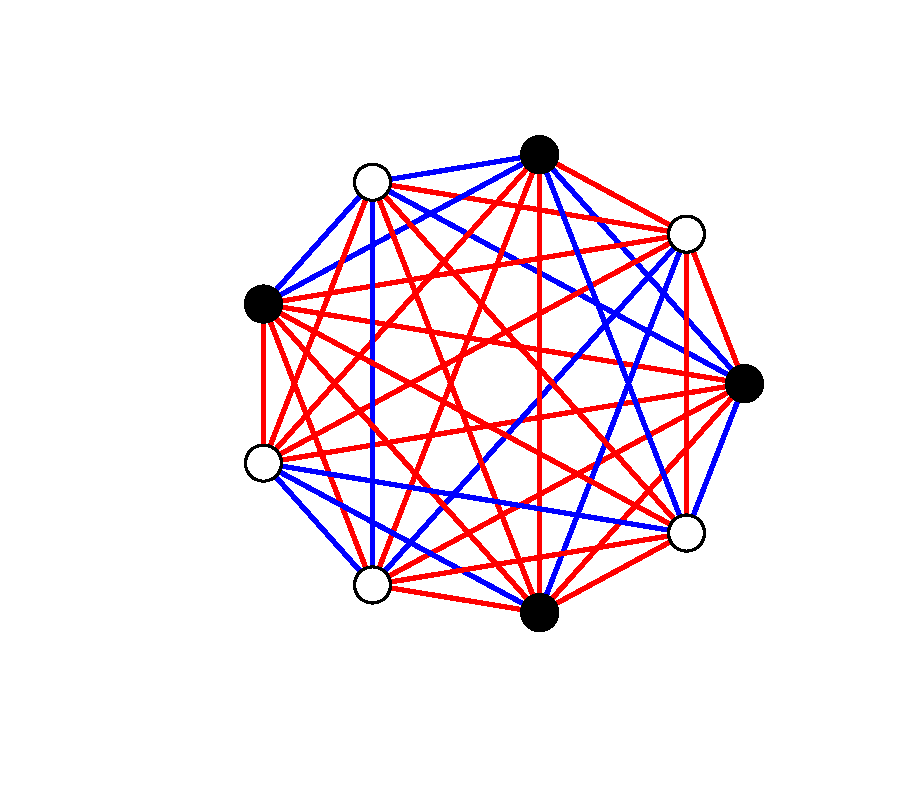
\includegraphics[width=.85\linewidth,clip,trim={100 70 70 60}]{images/ising_example}
\caption{Example of a fully connected Ising model with random couplings.}
\label{gr:ising}
\end{figure}

More generally, we could imagine that each of the spins has a particular bias given by an indexed local field $h_{\rm i}$ as well as particular interactions with neighbors $J_{\rm ij}$. The corresponding Hamiltonian is
\begin{align}
	E &= -\sum_{\rm \br{ij}} J_{\rm ij}\si\sj -\sum_{\rm i=1}^Nh_{\rm i}\si
\end{align}
and as mentioned before states with lower energy are more likely so spin tend to orient along the direction of the local field $h_{\rm i}^{\rm local} = \sum_{\rm j}J_{\rm ij}\sj +h_{\rm i}$. 

The Ising model corresponds to a pairwise maximum entropy model.
Fixing the the magnetizations and pairwise correlations to those observed in the data
\begin{align}
	\br{\si}_{\rm data} &= \br{\si}\\
	\br{\si\sj}_{\rm data} &= \br{\si\sj}
\end{align}
Constructing the Langrangian from Eq ??
\begin{align}
	\mathcal{L}[p] &= -\sum_s p(s)\log p(s) +\sum_{\rm \br{ij}} J_{\rm ij}\br{\si\sj} +\sum_{\rm i=1}^Nh_{\rm i}\br{\si}\\
	\frac{\partial\mathcal{L}[p]}{\partial p(s)} &= -\log p(s)-1 +\sum_{\rm \br{ij}} J_{\rm ij}\si\sj +\sum_{\rm i=1}^Nh_{\rm i}\si\\
	\log p(s) &= -1 +\sum_{\rm \br{ij}} J_{\rm ij}\si\sj +\sum_{\rm i=1}^Nh_{\rm i}\si\\
	p(s) &= \left.e^{-E(s)}\right/Z\\
\intertext{where to enforce normalization of the probability distribution $\sum_s p(s) = 1$,}
	Z &= \sum_s e^{-E(s)}
\end{align}
Thus, the resulting model is exactly the Ising model mentioned earlier.

%Imagine that you have a system with $n$ components that have been sampled many times. To be more specific, we'll take $n=9$ voters on the US Supreme Court that either vote with in the majority, the winning coalition, or in the minority. [More generally, we could think some like gene expression levels in a cell a coarse-grained representation where relatively high or low expression can be represented by a binary variable. Of course, we don't have to restrict ourselves to binary variables \cite{Lezon:2006ws}.]
%The primary difficulty for solving probabilistic models is calculating the normalization because of the size of the state space. Most of the methods below involve avoiding that problem in the first place (Monte Carlo sampling, MCH) or approximations to drastically reduce the state space (pseudolikelihood, adaptive cluster expansion).


\section{Exact enumeration}
The na\"{i}ve approach is to write the equations from Eq \ref{eq:dkl deriv} directly:
\begin{align}
	\br{f_{\rm k}} &= -\frac{\partial \ln Z}{\partial \lambda_{\rm k}}
\end{align}
Matching these with the data $\br{f_k}_{\rm data}$ is the purview of any standard optimization algorithm. Clearly, this approach does not scale well because the number of terms in the partition function grows exponentially with system size. For relatively small systems $n\leq15$, however, this approach is feasible on a typical desktop computer.
%[Simple example with logical gates?]

For the Ising model, the first step in the algorithm for writing down the equations is $\mathcal{O}(K^2 2^{N})$ where $K$ is the number of constraints and $N$ the number of spins. In the second step, each evaluation of the objective in the minimization algorithm will be of the same order.

The {\tt Exact} class supplies methods for writing Eqs \ref{eq:fk-fk} into a file and solving them with the {\tt scipy.optimize} library.


\section{Monte Carlo methods}
Perhaps the most straightforward and most expensive computational approach is to use Monte Carlo Markov Chain sampling to approximate the distribution and adjust the parameters appropriately after each step. [For details about MCMC methods see Appendix A and \cite{MacKay:2005wc}.] The magic behind MCMC approaches is that only relative probabilities of states need to be known to return a sample of the distribution. Thus, we no longer need to calculate the partition function, but can instead compute the difference in energy between two states.

The simplest MCMC algorithm is to generate a sample to estimate the constraints $\br{f_{\rm k}}$ from the current set of parameters and then to implement a learning rule to adjust the parameters. This can be combined with a variety of stochastic gradient descent methods to reduce the number of sampling steps. The particular technique implemented in CONIII is the Monte Carlo Histogram method \cite{Broderick:2007wq}.

Since the sampling step is expensive, the idea behind Monte Carlo histogram is to reuse a sample for more than one gradient descent step because we can predict how the distribution will change if we modify the parameters slightly \cite{Broderick:2007wq}. Given that we have a sample with probability distribution $p_s$ generated with parameters $\lambda_{\rm k}$, we would like to estimate the distribution $p_s'$ from parameters $\lambda_{\rm k}' = \lambda_{\rm k}+\Delta\lambda_{\rm k}$.
\begin{align}
	p_s' &= \frac{p'_s}{p_s}p_s\\
		&= \frac{Z}{Z'}e^{\sum_k \Delta\lambda_k f_k(s)} p_s\\
\intertext{To estimate the average,}
	\sum_s p_s' f_k(s) &= \frac{Z}{Z'} \sum_s p_s e^{\sum_k \Delta\lambda_k f_k(s)} f_k(s)\\
\intertext{But we have a sampled approximation to $p$.}
	\br{f_k}' &= \frac{Z}{Z'} \br{e^{\sum_k \Delta\lambda_k f_k(s)} f_k(s)}_{\rm sample}
\end{align}
Likewise, the ratio of the partition function can be estimated
\begin{align}
	\frac{Z}{Z'} \approx 1\left/\br{e^{\sum_k \Delta\lambda_k f_k(s)}}_{\rm sample}\right.
\end{align}

The main difficulty with MCH is choosing a learning rule for how to update the Lagrangian multipliers $\{\lambda_k\}$ at each iteration while being careful to stay within the bounds of a reasonable extrapolation. One suggestion is to update the parameters with some inertia
\begin{align}
	\Delta\lambda_k(t+1) &= \Delta \lambda_k(t) + \eta \Delta\lambda_k(t-1)\label{eq:mch learn1}\\
	\Delta \lambda_k(t) &= \epsilon\left(\br{f_k}'-\br{f_k}\right)\label{eq:mch learn2}
\end{align}
This has the correct fixed points. One suggestion is to shrink $\epsilon$ exponentially with the number of iterations. In the code, there are more parameters $\Delta\lambda_{\rm max}$ and $\Delta\lambda_{\rm norm}\sum_k \sqrt{\Delta\lambda_{\rm k}^2}$ that restrict. Another heuristic is to begin with estimates on a small data set and increase the size of the data set as we refine our estimates of the parameters.

Typically, one must check in on the progress of the algorithm to tune the various parameters. If the extrapolation steps or the gradient steps are too large, the algorithm will fail to converge (or may even start diverging).

The runtime for the sampling step is proportional to the number of samples $n_{\rm sample}$, number of MCMC iterations $n_{MC}$, the number of constraints $K$:
$\mathcal{O}(n_{\rm MC} n_{\rm sample} K)$, whereas the MCH estimate is relatively quick $\mathcal{O}(n_{\rm sample}n_{\rm MCH}K)$ because the number of MCH approximation steps is much smaller than the number of MCMC sampling iterations $n_{\rm MCH}<<n_{\rm MC}$. What is the runtime for the learning rules Eqs \ref{eq:mch learn1} and \ref{eq:mch learn2}?
For the Ising model, $K\sim N^2$, the system size squared.

MCH is implemented in the {\tt MCH} class.

\section{Pseudolikelihood}
The pseudolikelihood approach is an analytic approximation to the likelihood that drastically reduces the computational complexity of the problem and is exact in the thermodynamic limit \cite{Aurell:2012hi}. We maximize the conditional probability 
\begin{align}
	p\left(\sigma_{\rm i}|\boldsymbol{\sigma}_{\backslash \rm i};h,J\right) &= \left( 1+e^{-2\sigma_{\rm i} \left(h_{\rm i}+\sum_{j\neq i}J_{\rm ij}\sj\right)} \right)^{-1}
\end{align}

The objective consists of maximizing the conditional likelihood the set of parameters that correspond to the ith spin
\begin{align}
	f(h_{\rm i},\bs{J}_{\rm i}) &= \sum_{\rm r=1}^R \ln p\left(\left.\sigma_{\rm i}^{(r)}\right|\bs{\sigma}_{\backslash\rm i}^{(r)}\right)
\end{align}
summed over all data points indexed by $r$.
In the limit where the ensemble is well sampled, the average over the data can be replaced by an average over the ensemble
\begin{align}
	f(h_{\rm i},\bs{J}_{\rm i}) &= \sum_{\bs{\sigma}} \ln p\left(\left.\sigma_{\rm i}^{(r)}\right|\bs{\sigma}_{\backslash\rm i}^{(r)}\right)p(\bs{\sigma};h,J)\\
\intertext{At maximum likelihood,}
	\frac{\partial f}{\partial J_{\rm ij}} &= \sum_{\bs{\sigma}} \ln p\left(\left.\sigma_{\rm i}^{(r)}\right|\bs{\sigma}_{\backslash\rm i}^{(r)}\right)p(\bs{\sigma};h,J)\\
	0 &=
\end{align}

Each iteration goes like $O(RN^2)$.

We have implemented pseudolikelihood for the Ising model as detailed in \cite{Aurell:2012hi} in {\tt Pseudo}.

\section{Minimum Probability Flow}
Minimum probability flow involves analytically approximating how the probability distribution \textit{changes} as we modify the \textit{configurations} \cite{SohlDickstein:2011im}. In the methods so far mentioned, the approach has been to maximize the objective (the likelihood function) by immediately taking the derivative with respect to the parameters. With MPF, we first posit a set of dynamics that will lead the data distribution to equilibrate to that of the model. When these distributions are equivalent, then there is no ``probability flow'' between them. This technique is closely related to score matching where instead we have continuous state spaces and can directly take the derivative with respect to the states without specifying dynamics \cite{Hyvarinen:2007ed}.

As before, we start with minimizing the Kullback-Leibler divergence, but instead of taking the derivative with respect to the parameters, we first ask how the probability flows between the model and data if the dynamics are run for an infinitesimal amount of time $\epsilon$, the idea being that the relative difference between the probability distributions are minimized with optimal parameters.
\begin{align}
	\partial_t D_{KL}(p^{(0)}||p^{(t)}\left(\{\lambda_k\}\right)) &= \sum_{\rm i \not\in \mathcal{D}} \dot{p}_{\rm i}(\lambda_k)\\
	K(\{\lambda_{\rm k}\}) &= \sum_{\rm i \not\in \mathcal{D}} \dot{p}_{\rm i}(\lambda_k)
\end{align}

Monte Carlo dynamics (satisfying ergodicity and detailed balance) would lead to equilibration of the two distributions, so the suggestion of in \cite{SohlDickstein:2011im} is
\begin{align}
	\dot{p}_{\rm i} &= \sum_{j\neq i} \Gamma_{\rm ij} p_{\rm j} -\sum_{\rm j\neq i} \Gamma_{\rm ji} p_{\rm j}
\end{align}
with transition probabilities $\Gamma_{\rm ij} = g_{\rm ij}\exp\left[ \frac{1}{2}\left( E_{\rm j}-E_{\rm i} \right) \right]$ from state j to state i. The connectivity matrix $g_{\rm ij}$ specifies whether there is edge between states i and j such that probability can flow between them. By choosing a sparse $g_{\rm ij}$ while not breaking ergodicity, we drastically reduce the computational cost of calculating the objective function.

Finally, we must find the minimum of the objective function
\begin{align}
	K(\{\lambda_{\rm k}\}) &= \sum_{\rm i \not\in \mathcal{D}} \dot{p}_{\rm i}(\lambda_k)
\end{align}

MPF satisfies a number of useful properties:

[Typically with large systems, numerical precision errors can become a problem because of the exponential form of $p(\lambda_{\rm k})$. By taking the logarithm of the objective $K$ can be crucial to a working implementation.]

MPF is implemented in the {\tt MPF} class.


\section{Regularization to avoid overfitting}

Besides the computational complexity of locating best-fit parameters,
a fundamental problem in any model inference method is that uncertainty coming
from the finiteness of data translates into uncertainties in parameters.
The straightforward answer to this problem is to take more data---in a pairwise
maximum entropy problem, we might insist that we have enough samples to well-constrain
the correlation between every pair of individuals.  But it is not always possible
to take enough data.  For instance, in a social system in which we are trying to
measure stable social structure that lasts on the order of months, there are only
a finite number of social interactions that occur over those months, which may
not be enough to tightly constrain parameters.

The danger in naively searching for a best-fit solution in a data-poor situation
is overfitting, or erroneously finding patterns in the finite-sample noise.
One way to avoid overfitting is regularization:
restricting the search space in some principled way so that more complicated
solutions are disallowed.  We then check that the regularized solutions fit the
data within expected statistical fluctuations.  If not, a more lax regularization
can be used to allow more complicated solutions that are able to fit the
remaining signal in the data.

We will motivate the next two approaches to maximum entropy fitting in terms
of regularization.

[This section might be tightened a bit more.  For one, I am somewhat confused as
to whether the entire maximum entropy approach might be motivated in this
way---starting with few constraints and adding the possibility of higher order
constraints until the model fits well enough.]


\section{Mean-field methods}
[I'm imagining that we neatly tie together the different techniques. As far as I know, they're all different approaches and no one's done a real good job relating one technique to another. It's easy enough to go read a bunch of different papers about each method, but it's not so clear why one is preferable over another.]

[Analytic approximations simplify the equations to an extent where they are tractable.]

One attractively simple and efficient version of the regularized approach starts
with mean-field theory.  In the inverse Ising problem, mean-field theory is equivalent
to treating each binary individual as instead having a continuously varying state
(corresponding to its mean value).  The inverse problem then turns into simply inverting
the correlation matrix $C$: \cite{CocMon12}
\begin{equation}
\label{meanFieldSolution}
J^{\mathrm{mean-field}}_{k\ell} =
    - \frac{ (C^{-1})_{k\ell} }{ \sqrt{p_k(1-p_k)p_\ell(1-p_\ell)} },
\end{equation}
where
\begin{equation}
C_{k\ell} = \frac{ p_{k\ell} - p_k p_\ell }{ \sqrt{p_k(1-p_k)p_\ell(1-p_\ell)} },
\end{equation}
and where $p_k$ corresponds to the frequency of individual $k$ being
in the active ($+1$) state and $p_{k\ell}$ is the frequency of the pair
$k$ and $\ell$ being simultanously in the active state.

A simple regularization scheme in this case is to discourage large values in the interaction
matrix $J$.  This corresponds to putting more weight on solutions that are closer to
the case with no interactions (independent individuals).  A particularly convenient form
adds the following term, quadratic in $J$, to the negative log-likelihood:
\begin{equation}
\gamma \sum_i \sum_{j > i} J_{ij}^2 p_i (1-p_i) p_j (1-p_j).
\end{equation}
In this case, the regularized version of the mean-field solution in \eqref{meanFieldSolution}
can be solved analytically, with the slowest computational step coming from the inversion
of the correlation matrix.  For details, see Refs.~\cite{DanKraFla17,BarCoc13}.

The idea is then to vary the regularization strength $\gamma$ to move between the
non-interacting case ($\gamma \rightarrow \infty$) and the naively calculated
mean-field solution \eqref{meanFieldSolution} ($\gamma \rightarrow 0$).
While there is no guarantee that varying this one parameter will produce solutions that are
good enough to ``fit within error bars,'' this approach has been successful in at least
one case of fitting social interactions \cite{DanKraFla17}.

This is implemented in {\tt RegularizedMeanField}.



\section{Cluster expansions}

Adaptive cluster expansion \cite{CocMon11,CocMon12,BarCoc13}
iteratively calculates terms in the
cluster expansion of the entropy $S$:
\begin{equation}
S = \sum_\Gamma \Delta S_\Gamma,
\end{equation}
where the sum is over clusters $\Gamma$ and in the exact case
includes all $2^N - 1$ possible nonempty subsets of individuals in the system.
\footnote{In the simplest version of the expansion,
one expands around $S=0$.  In some cases it can be more advantageous to write the
expansion around $S-S_0$, where $S_0$ is a reference entropy corresponding to
an easily calculated case such as
the independent individual solution or one of the mean-field solutions
described in the previous section \cite{BarCoc13}.}
The inverse Ising problem is solved independently
on each of the clusters, which can be done exactly when the
clusters are small.  These results are used to construct a full
interaction matrix $J$.
The expansion starts with small clusters and expands to use larger
clusters, neglecting any clusters whose
contribution $\Delta S_\Gamma$ to the entropy falls below a threshold.
To find the best solution that does not overfit,
the threshold is initially set at a large value and then lowered,
gradually including more clusters in the expansion, until samples from
the resulting $J$ fit the desired statistics of the data sufficiently well.

In Coniii, the selective cluster expansion method is implemented in the {\tt ClusterExpansion} class.

\section{Bethe/Kikuchi free energy/cavity methods}
Another approach involves a cluster-expansion of the free energy, also known as the cavity method. This has not yet been implemented in CONIII.

The cavity method involves use of the marginalized distribution.

\section{Samplers}
In CONIII, we have implemented two versions of the Metropolis algorithm. One is specific to the Ising model {\tt MCIsing} and the other {\tt MC} can sample a system as long as the function for calculating the energy is suppiled by the user.

\subsection{How to validate a maxent model}
The logic behind maxent is that by fixing some aspects of the probability distribution, the rest of the distribution has been well characterized.
Another way to put this is to say that the distributions are well-peaked about the constraints. If this condition does not hold, the constraints are not useful.

Maxent is not a typical fitting method where the optimal parameters are sought such that the model is as good as possible. Instead, we specify which aspects of the system we think are important and the resulting ``parameters'' come from the maximum entropy principle.

Thus, one way to test the model is to consider how well we do in predicting the rest of the distribution. If the rest of the distribution is not well fit, certainly we must go back and reconsider which constraints to impose. On the other hand, finding that the rest of the probability distribution is fit well does not necessarily mean we have found the right model.

%\section{Why not maximum entropy?}



\appendix

\section{The microcanonical ensemble and maximum entropy}
The conventional textbook in statistical mechanics first introduces the concept of entropy as a way of counting the phase volume available to the system at a given energy
\begin{align}
	S(E) &= k_B \log\Omega(E)
\end{align}
where $k_B$ is Boltzmann's constant and $\Omega$ the number of states between $E$ and $E+\delta E$. Temperature is defined as
\begin{align}
	\frac{1}{T} &= \frac{\partial S}{\partial E}
\end{align}

 begins with the concept of a small system coupled to a heat bath. In this limit, we can linearly expand thermodynamic quantities about the energy of the bath $E_{\rm bath} = E-E_s$
\begin{align}
	S_{\rm bath}(E-E_s) &\approx S_{\rm bath}(E) -E_s\left.\frac{\partial S}{\partial E_s}\right|_{E-E_s}\\
		&= S_{\rm bath}(E) -\frac{E_s}{T}\\
	e^{S_{\rm bath}(E-E_s)/k_B} &= e^{S_{\rm bath}(E)/k_B} e^{-E_s/k_BT}
\intertext{Since the entropy is proportional to the density of states at a particular energy $E_s$, Eq ?? corresponds to}
	p(E_s) &= e^{-E_s/k_BT}/Z
\end{align}
With partition function $Z$. In other words, the Gibbs measure takes exponential form. Eq ?? can be rewritten in terms of free energy
\begin{align}
	\log p(E_s) &= -E_s/k_BT -\log(Z)
\intertext{Averaging both sides over all energy configurations and rearranging}
	-k_B T\log Z &= \sum_s p(E_s) E_s +k_BT\sum_s p(E_s)\log p(E_s)
\intertext{Remembering the fundamental postulate of statistical mechanics that all states are equally likely}
	-k_BT\log Z &= \br{E_s} - TS\\
	F &= \br{E_s} -TS
\end{align}
This equation tells us how the Helmholtz free energy is related to the internal energy and the entropy of the system.

When we say that free energy is minimized for a system with Hamiltonian $E_s$ at equilibrium, we are equivalently saying that entropy is maximized. Entropy maximization is the crux of statistical physics models.
%A more colloquial way of stating this is that statistical mechanics models produce a distribution that is as ``spread out'' as possible given a particular form to the energy function and a temperature.

\section{Notes on Monte Carlo Markov Chain sampling}
The key points behind MCMC sampling is ergodicity and detailed balance. Ergodicity just means that we can get from one state to another in a finite number of steps, and this ensures that we don't get stuck in a few states. Detailed balance is a sufficient but not necessary condition (stronger than needed) for ensuring that the equilibrium distribution matches the distribution that we seek. There are some specialized algorithms that don't satisfy detailed balance but do produce the desired distribution.

To check whether an algorithm works, one must prove that both these conditions are satisfied. Ergodicity is usually trivial. Typically, we write down the condition for detailed balance for any two states $a$ and $b$,
\begin{align}
	p(a|b)p(b) &= p(b|a)p(a) \\
	p(b)/p(a) &= p(b|a)/p(a|b) \\
	e^{-(E_b-E_a)} &= 
\end{align}
A reasonable way to do this would be to take $p(b|a) = e^{-(E_b-E_a)}$ and $p(a|b) = 1$ when $E_b>E_a$.

\begin{align}
	p_a\,T(a\rightarrow b)A(a\rightarrow b) &= p_b\,T(b\rightarrow a)A(b\rightarrow a)\\
	p_a/p_b &= T(b\rightarrow a)A(b\rightarrow a)/T(a\rightarrow b)A(a\rightarrow b)
\end{align}
where $T$ is the transition probability and $A$ is the acceptance probability. For a Boltzmann type model, this means that this ratio must be equal to $\exp(-\beta(E_a-E_b))$.

\subsection{Swendsen-Wang}
As an example, we consider the Swendsen-Wang cluster algorithm. In this algorithm, the first step is to form bonds between like spins (to grow clusters) then we flip to any configuration permitted by the current bond structure which is uniform. If you work through the calculations (GNB V pg 81), you will find that the probability of transitioning between states depend on the bonds that could have formed between like spins but didn't, and this is equal to the energy difference between the states.

\subsection{Wolff}
Another example is the Wolff algorithm (see GNB V pg 83) which is like the SW algorithm except that only a single cluster is build and flipped at a time with probability 1, i.e. the acceptance probability is 1 in the original algorithm. We start with any random site as the initial spin then we build a cluster spreading out from that spin to its nearest neighbors where the choose the probability of choosing a neighbor to be $1-\exp(-2J_{ij})$.

The random fields can be accounted for in the acceptance probabilities (so the probability of a cluster flipping is no longer 1). Working through the math, you will find that the cluster growth accounts for the ratio of the energies that come from the couplings but to account for the fields, the probability of a particular orientation of the clusters has to be
\begin{align}
	p(\Sigma_n) &\propto \exp\left(\sum_i h_i\sigma_i\right)
\end{align}
which we can easily simulate using something like the Metropolis algorithm. Obviously, this will increase the correlation time between samples because we will not always accept a cluster flip. This can be especially problematic when the clusters become large and have similar fields, but as long as the sum of the distribution of local fields for spins in a cluster is symmetric about 0, this will not be too slow. Certainly, it is faster than any local flip algorithm.

A simple example that I worked through is with 4 spins and the transition probability between two different states. Here, we can easily enumerate all possible ways of transitioning between these two states using the Wolff algorithm.

\section{Replica exchange Monte Carlo (REMC)}
REMC simulates multiple replicas of the system at different temperatures simulaneously and allow states to be exchanged between them. The idea is that an energy barrier may be very difficult to cross below a certain critical temperature, but there may be a trajectory allowed by diffusing through higher temperatures to cross the boundary.

Instead of considering the ensemble of a single system, we consider the ensemble of multiple independent systems. Thus, the joint probability distribution on the extended state space is
\begin{align}
	p(\sigma,\beta_n).
\end{align}
where $\beta_n = 1/T_n$ is the inverse temperature.

The simplest possible assumption for the shape of this distribution would be that the probability of occupying any particular temperature $\beta_n$ is uniform $p(n) = 1/N_T$. It turns out that this is optimal according to some criterion (see citation in Kerler and Rehberg). Note that this is not the same as just simulating a set of replicas for which the partition funtion would be
\begin{align}
	Z &= \prod_{m} \sum_\sigma \exp\left[ -\beta_m H(\sigma) \right] \label{eq:equi Z}
\end{align}
This is for the obvious reason that the average energy is a function of $T$ so a simulation of Eq \ref{eq:equi Z} would spend much more time exploring lower temperatures than higher temperatures. This makes it difficult to have the system use higher energy states to cross energy barriers. 

So instead of Eq \ref{eq:equi Z}, we can include a term $g_n$ to compensate
\begin{align}
	Z &= \prod_{m} \sum_\sigma \exp\left[ -\beta_m H(\sigma) +g_m \right]
\end{align}
How do we find $g_n$?

Under the assumption that the probability $p(n)$ is a constant,
\begin{align}
	p(n) &= e^{g_n} \sum_\sigma \exp\left[ -\beta_n H(\sigma) \right]/Z\\
	g_n &= \log[p(n)\,Z] + \tilde{Z}_n\\
	g_n &\rightarrow \tilde{Z}_n
\end{align}
(remembering that constants don't matter in the relation between energy and probability) where 
\begin{align}
	\tilde{Z}_n &= \sum_\sigma \exp\left[ -\beta_n H(\sigma) \right]
\end{align}
One way to find the $g_n$ that satisfy this condition is to come up with an iterative algorithm that converges to a fixed point. One suggestion is to estimate $g_n$ by reweighting the distributions from adjacent replicas.

Now, it remains to find a set of $\beta_n$ that is optimal for simulating relaxing into equilibrium quickly. One suggestion to make the algorithm spend an equal amount of time at each temperature. Kerler and Rehberg suggest a method.

\bibliography{guide}

\end{document}  
